\section{Interference Bound Function}
 % We will also apply an optimization technique to further improve the performance of the test because the resource consumed by $\tau$ before $r_{i,x}$ or $P_{i,x}$ can not be greater than $r_{i,x}$ or $P_{i,x}$, respectively. Thus here we also derive  $f_i^1(\tau_j,t')$ and $f_i^2(\tau_j,t')$ which denote the maximum possible resource consumed by  $\tau_j$ after $r_{i,x}$ and $P_{i,x}$, respectively.  

% For static priority scheduling, $f_i(\tau_j,t')$ returns the maximum cumulative execution requirement by jobs of $\tau_j$ that have their release time within the time interval $[0,t']$. However this is not the case for dual priority scheduling  as shown in the following example.
% \begin{example}
% As shown in the Figure~1, when $r_{i,x}\leq t'\leq P_{i,x}$, the execution requirement of $J_{j,y}$ is $C_j$ because $\tau_i$  would execute only after $J_{j,y}$ finishes. However, when $P_{i,x}\leq t'\leq P_{j,x}$,  the time $J_{j,y}$ deny processor from $\tau_i$ is equal the time that $J_{j,y}$ has already executed by $P_{i,x}$, because $\tau_i$ has higher priority than $\tau_j$ during $[P_{i,x},P_{j,y}]$. 
% \begin{figure}[h!]
%  \centering
% 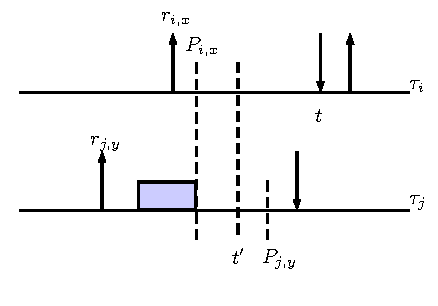
\includegraphics[scale=1]{Figure/E1}  
% \caption{Example One}
%   \label{fig:p3}
% \end{figure}
% \end{example}
% From the above example we know that the exact time that $\tau_j$ has executed by $t'$ in fact depends the release pattern of all the tasks in the system. Meanwhile the release pattern of each task (including $\tau_i$) would influence each other and hence it is hard which patten would maximize $F(\tau_i,t,t')$.






When calculating $f_i(\tau_j,t',t)$, we ignore the interference from the other tasks on $\tau_j$ except $J_{i,x}$. Thus we have the following lemma.
\begin{lemma}[Maximum Execution]
\label{lemma:1}
$f_i(\tau_j,t',t)$ is maximized when  $J_{j,1}$ is released at $0$ and all jobs are released as soon as possible with period $T_j$, and each job of $\tau_j$ executes as early as possible as long as it has higher priority than $J_{i,x}$.
\end{lemma}
\begin{proof}
When  $J_{j,1}$ is released at $0$ and all jobs are released as soon as possible with period $T_j$, the number of jobs that released during $[0,t']$ is maximized. Meanwhile as we either shift the release pattern left or right,  the total execution would only decrease or stay the same.
\end{proof}


\begin{itemize}
	\item $J_{j,y}$ is the job that has its release time $r_{i,y}\leq t'<r_{i,y}+T_j$. Since $r_{j,1}=0$, we know $r_{j,y}=\lfloor \frac{t'}{T_j}\rfloor\times T_j$
	\item $[a]_0=\max(a,0)$
\end{itemize}

With Lemma~\ref{lemma:1}, we can easily calculate $f_i(\tau_j,t',t)$, and in the following section, we present the detailed equations.
\subsection{$f_i(\tau_j,t',t)$ when $j<i$}
We first consider the case when index $j$ is smaller than index $i$ which means $\tau_j$ has higher origin priority than $\tau_i$. Thus if  $J_{j,y}$ is still active, $J_{i,x}$ would not  execute unless it is during the interval $[P_{i,x}, P_{j,y}]$ (if $P_{i,x}<P_{j,y}$).


\textbf{Case 1 ( $P_{j,y}\leq P_{i,x}$)} as shown in  Figure~\ref{fig:case1}: Job $J_{i,x}$ always has lower priority than  $J_{j,y}$. Thus   the maximum possible resource consumed by $\tau_{j}$  before $t'$ is  bounded by
	\begin{align*}
		f_i(\tau_j,t')=\lfloor \frac{t'}{T_j}\rfloor.C_j +\min\left(C_j,t'-r_{j,y}\right)
	\end{align*}
 

\begin{figure}[h!]
 \centering
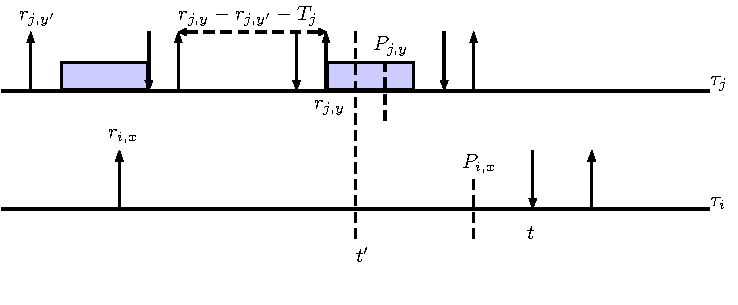
\includegraphics[scale=0.7]{Figure/C1}  
\caption{$ P_{j,y}\leq P_{i,x}$}
  \label{fig:case1}
\end{figure}






\begin{figure}[h!]
 \centering
\includegraphics[scale=0.7]{Figure/C2}  
\caption{$P_{j,y}> P_{i,x}$}
  \label{fig:case2}
\end{figure}

\textbf{Case 2} ($P_{j,y}> P_{i,x}$):~as shown in  Figure~\ref{fig:case2}, $J_{i,x}$ has higher priority than $J_{j,y}$'s  during $[\max(r_{j,y},P_{i,x}),P_{j,y}]$ (if $P_{i,x}\leq P_{j,y}$). Thus  $J_{j,y}$ can not execute  during $[\max(r_{j,y},P_{i,x}),P_j]$ unless $J_{i,x}$ has already finished. Thus we have
	\begin{align*}
		&f_i(\tau_j,t')=\lfloor \frac{t'}{T_j}\rfloor.C_j +
\\&\min\left(C_j,\!t'\!-\!r_{j,y}\!-\!\left(\min(t'\!,\!P_{j,y})\!-\!\max(r_{j,y},\!P_{i,x})\right)\right)
		\end{align*}




% 
\subsection{$f_i(\tau_j,t')$ when $j> i$}
 
\textbf{Case 1.1} ($P_{i,x}\leq P_{j,y}\wedge r_{j,y}\leq r_{i,x}$): as shown in  Figure~\ref{fig:case3}, $\tau_j$ may execute during $[r_{j,y},r_{i,x}]$, but $\tau_j$ would not execute after $r_{i,x}$  unless $\tau_i$ has finished.

	\begin{figure}[h!]
 \centering
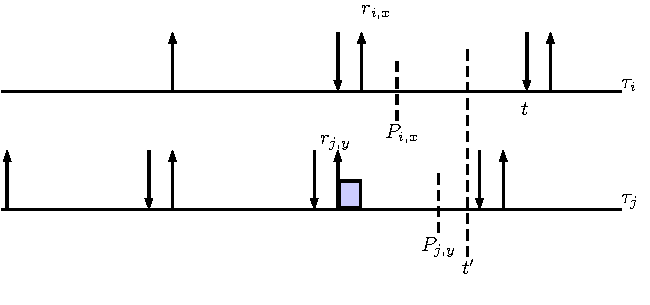
\includegraphics[scale=0.7]{Figure/C3}  
\caption{$P_i\leq P_j\wedge r_j\leq r_i$}
  \label{fig:case3}
\end{figure}
		\begin{align*}
		f_i(\tau_j,t')=\lfloor \frac{t'}{T_j}\rfloor\times C_j+\min(C_j,r_{i,x}-r_{j,y})
	\end{align*}
% However $J_{j,y}$ would never execute after $r_{i,x}$, and hence we have
% \begin{align*}
% &rbf_{i}^1(\tau_j,t')=\min(C_j,r_{i,x}-r_{j,y})
% \end{align*}


% \begin{align*}
% \begin{split}
% rbf_{i}^2(\tau_j,t')=0
% \end{split}
% \end{align*}


\textbf{Case 1.2} ($P_{i,x}\leq P_{j,y}\wedge r_{j,y}> r_{i,x}$): as shown in  Figure~\ref{fig:case4},  $J_{j,y}$ would not execute unless $\tau_i$ has completed. Thus we have
\begin{align*}
		f_i(\tau_j,t')=\lfloor \frac{t'}{T_j}\rfloor\times C_j
\end{align*}

\begin{figure}[h!]
 \centering
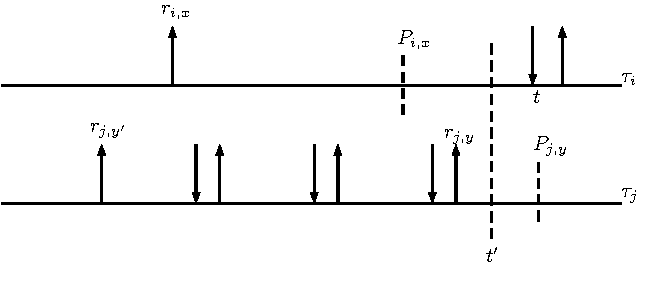
\includegraphics[scale=0.7]{Figure/C31}  
\caption{$P_{i,x}\leq P_{j,y}\wedge r_{j,y}> r_{i,x}$}
  \label{fig:case4}
\end{figure}



\textbf{Case 2.1} ($P_{i,x}>P_{j,y}\wedge r_{j,y}\leq r_{i,x}$): as shown in  Figure~\ref{fig:case5}, after $r_{i,x}$,  $J_{j,y}$ can only execute during $[\max(r_{i,x},P_{j,y}),	\min(t',P_{i,x})]$
	\begin{align*}
		&f_i(\tau_j,t')=\lfloor \frac{t'}{T_j}\rfloor\times C_j+\\
		&\min\left(C_j,r_{i,x}-r_{j,y}+[\min(t',P_{i,x})-\max(P_{j,y},r_{i,x})]_0\right)
	\end{align*}


\begin{figure}[h!]
 \centering
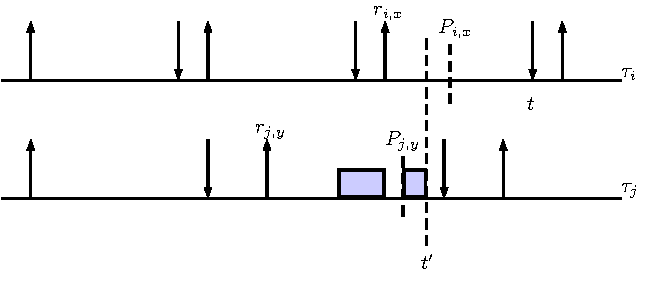
\includegraphics[scale=0.7]{Figure/C4}  
\caption{$P_{i,x}>P_{j,y}\wedge r_{j,y}\leq r_{i,x}$}
  \label{fig:case5}
\end{figure}

\begin{figure}[h!]
 \centering
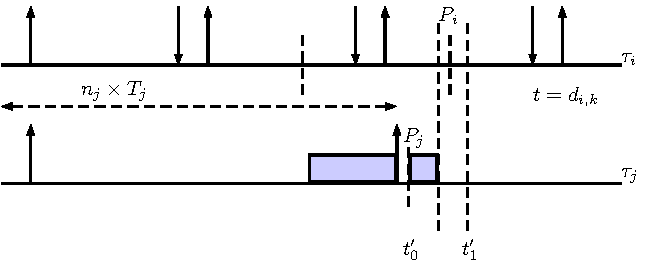
\includegraphics[scale=0.7]{Figure/C41}  
\caption{$P_{i,x}>P_{j,y}\wedge r_{j,y}> r_{i,x} $}
  \label{fig:case6}
\end{figure}

\textbf{Case 2.2} ($P_{i,x}>P_{j,y}\wedge r_{j,y}> r_{i,x}$): as shown in  Figure~\ref{fig:case6}, $J_{j,y}$ would only execute during $[P_{j,y},P_{i,x}]$ before $J_{i,x}$ finishes. Thus we have
\begin{align*}
	f_i(\tau_j,t')=\lfloor \frac{t'}{T_j}\rfloor.C_j+\min\left(C_j,[\min(t',P_{i,x})-P_{j,y}]_0\right)
\end{align*}






